\section{Static Network Conditions}\label{sec:static}

In this section, we study the effect of network capacity on VCA performance.

\paragraph{Method}: We conduct a series of experiments, each consisting of a
2.5-minute call between two clients, V1 and V2 (as described in
Section~\ref{subsec:setup}), under a specific shaping level. We conduct two
sets of experiments, shaping first the uplink and then the downlink.  We
constrain throughput to \{$0.3, 0.4, \dots, 1.4, 1.5, 2, 5, 10$\}~Mbps (in
each of the upstream and downstream directions). For each condition, we perform five 2.5-minute experiments; our
data show that due to relatively low variance in most observations, this
number of experiments is sufficient to achieve statistically significant
results.  For \zoom and \teams clients, we perform measurements both for
native clients as well as for browser-based clients, referred to as
\zoombrowser and \teamsbrowser, respectively. 

%% experiment setup
%% what is the experiment duration 
%% what bandwidth profiles are used 

% \tarun{Open questions: i) What about Team native client? ii) Audio performance? iii) Re-do \zoombrowser for 0.3 Mbps and 0.4 Mbps}



\subsection{Network Utilization}
\label{subsec:network_utilization}

\paragraph{Constrained upstream utilization}: Figure~\ref{subfig:uplink_bitrate} shows the
median sent network bitrate for different uplink capacities. We observe differences in upstream network
utilization among VCAs given the same available uplink network capacity. In
the case of a 10~Mbps uplink, for example, the average upstream utilization for
\teamsnative is $1.44$ Mbps whereas it is only $0.95$ for \meet and $0.77$
Mbps for \zoom. All three VCAs utilize the uplink efficiently (above 85\%)
when that link is constrained (0.8 Mbps or lower), although \meet's
bitrate is slightly higher than the other VCAs.  

\begin{table}[t]
\centering
\begin{tabular}{|c|c|c|}
\hline
\multirow{2}{*}{\textbf{VCA}} & 
    \multicolumn{2}{c|}{{\bf Utilization (Mbps)}} \\ 
    \cline{2-3} 
                              & Upstream                   & Downstream                  \\ \hline
Meet                          & 0.95                     & 0.84                      \\ 
Teams                         & 1.40                      & 1.86                      \\ 
Zoom                          & 0.78                     & 0.95                      \\ \hline
\end{tabular}
\caption{Unconstrained network utilization.}
\vspace{-1.5em}
\label{tab:vca_static}
\end{table}





\paragraph{Constrained downstream throughput}: We explored the effect of constrained
downstream capacity
on VCAs' network utilization. Figure~\ref{subfig:downlink_bitrate} shows this
result.
As with a constrained uplink, the VCAs differ in terms of their downlink
utilization under unconstrained link. The unconstrained downlink utilization
differs from unconstrained upstream utilization, as shown in
Table~\ref{tab:vca_static}. To better understand this phenomenon, we analyzed the traffic
captured from both clients. 

In the case of \teams, we found that the sent traffic from V1
is almost same as the received traffic at V2, and vice versa. 
We suspect the small
differences in upstream and downstream utilization may largely be due to the
variability in utilization across experiments in \teams, as is
also evident in the larger confidence intervals as compared to \zoom and \meet. 

In contrast, \zoom's utilization patterns were asymmetric: we found an
asymmetry in sent and received data rates at both clients. For instance, in a
single instance with 10~Mbps downlink shaping, V2 sent a median 0.85~Mbps and
V1 received a median 1.10 Mbps. Investigating this asymmetry further, we
discovered an interesting phenomenon: We found that \zoom uses a relay server
instead of direct communication. Additionally, related work by Nistico et
al.~\cite{nistico2020comparative} suggests that \zoom uses Forward Error
Correction (FEC) for error recovery. This is further supported by a related
patent from \zoom itself, which talks about a methodology to generate FEC data
at the server~\cite{liu2019error}. We suspect that the extra data may thus
correspond to FEC added by the relay server, leading to asymmetric upstream and
downstream utilization.  

\begin{figure*}[t]
	%\vspace{-10em}
    \begin{subfigure}[t]{0.33\textwidth}
    		\centering
        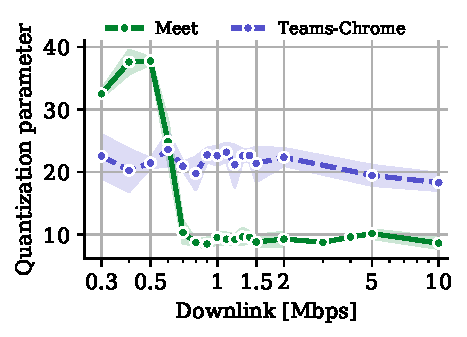
\includegraphics[width=\textwidth,keepaspectratio]{static/downlink_r_qpsum.pdf}
        \caption{Downlink - Quantization parameter}
 		\label{subfig:downlink_video_qp}
    \end{subfigure}%
    \hfill
	\begin{subfigure}[t]{0.33\textwidth}
        \centering
        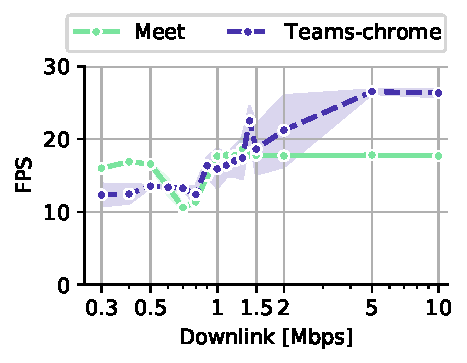
\includegraphics[width=\textwidth]{static/downlink_received_framesPerSecond.pdf}
    \caption{Downlink - Frames per second.}
    \label{subfig:downlink_frames_per_second}
    \end{subfigure}% 
    \hfill
	\begin{subfigure}[t]{0.33\textwidth}
        \centering
        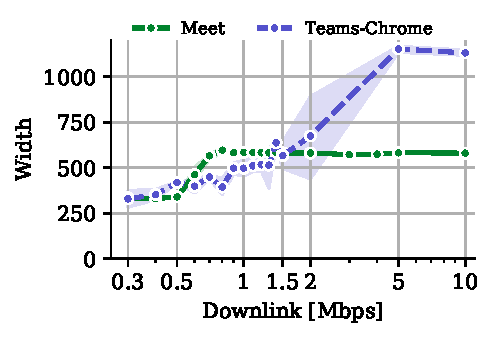
\includegraphics[width=\textwidth]{static/downlink_received_frameWidth.pdf}
    \caption{Downlink - Frame width.}
    \label{subfig:downlink_frame_width}
    \end{subfigure}
    \newline
        \begin{subfigure}[t]{0.33\textwidth}
    		\centering
        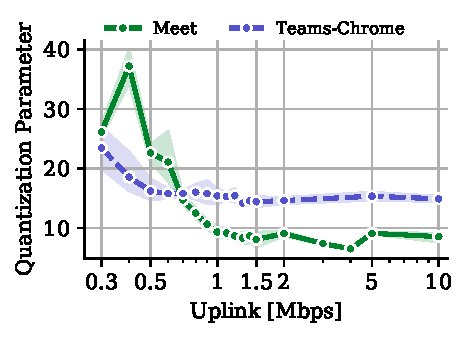
\includegraphics[width=\textwidth,keepaspectratio]{static/uplink_s_qpsum.pdf}
        \caption{Uplink - Quantization parameter.}
 		\label{subfig:uplink_video_qp}
    \end{subfigure}%
    \hfill
	\begin{subfigure}[t]{0.33\textwidth}
        \centering
        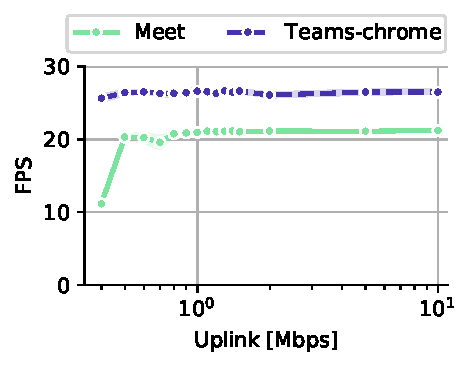
\includegraphics[width=\textwidth]{static/uplink_sent_framesPerSecond.pdf}
    \caption{Uplink - Frames per second.}
    \label{subfig:uplink_frames_per_second}
    \end{subfigure}% 
    \hfill
	\begin{subfigure}[t]{0.33\textwidth}   
        \centering
        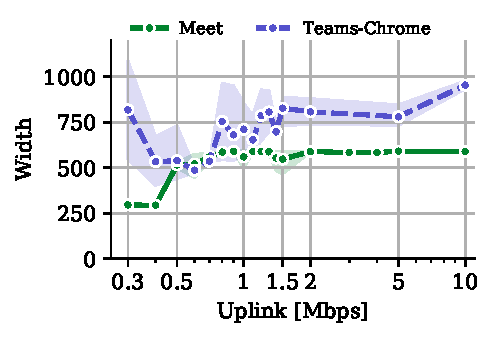
\includegraphics[width=\textwidth]{static/uplink_sent_frameWidth.pdf}
    \caption{Uplink - Frame width.}
    \label{subfig:uplink_frame_width}
    \end{subfigure}
	\caption{Video encoding parameters with 90\% confidence intervals under
    downstream and upstream throughput constraints.}
    \vspace{-1em}
	\label{fig:video_qual}
\end{figure*}

In addition to the asymmetric unconstrained utilization, \meet exhibits
markedly different behavior with a constrained downlink.
Specifically, the
network utilization with constrained downstream throughput (< 0.8 Mbps) is
only 39--70\%
(Figure~\ref{subfig:downlink_bitrate}), while it is more than $90\%$ in the
case of a constrained uplink (Figure~\ref{subfig:uplink_bitrate}). Upon
further exploration, we discovered that
\meet also uses a relay server, as well as
\textit{simulcast}, wherein the sender (V2) transmits multiple copies of the
video to the server, each at a different quality
level~\cite{nistico2020comparative}. The server then relays one of the quality
streams to V1 depending on the inferred available capacity of the server-V1
link. We observe two simultaneous video streams in our experiments, one at
320x180 and other at 640x360 resolution. When downstream throughput is
constrained, the relay
server cannot switch to a higher quality video and keeps sending at low
quality bitrate. This explains why \meet's network utilization at 0.5 Mbps is
only 0.19~Mbps, almost similar to its utilization at 0.3 Mbps.  The use of
simulcast also explains the higher upstream utilization as compared to
downstream utilization. 

\paragraph{Browser vs. native client utilization}:
Figure~\ref{subfig:uplink_browser} compares the upstream utilization of \zoom
and \teams between their respective native and Chrome clients. \zoom's
utilization is similar across the native and browser-based platforms; in
contrast, we find significant difference between \teams native and browser
client. When uplink capacity is shaped to 1~Mbps, the \teams-native client
uses 0.84 Mbps, whereas \teamsbrowser uses only 0.61 Mbps. We found a
similar difference between \teams-native and \teamsbrowser when downstream
throughput is constrained. 

\begin{figure}[t]
    \centering
    \begin{subfigure}[t]{0.4\textwidth}      
        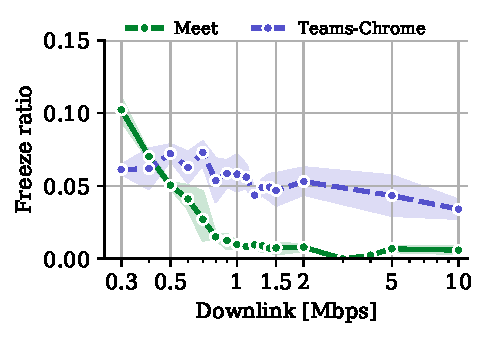
\includegraphics[width=\textwidth,keepaspectratio]{static/downlink_freezeRatio.pdf}
        \vspace{-1em}
        \caption{Downstream: Freeze ratio.}
 		\label{subfig:downlink_freeze_ratio}
    \end{subfigure}
	\begin{subfigure}[t]{0.4\textwidth}   
        \centering
        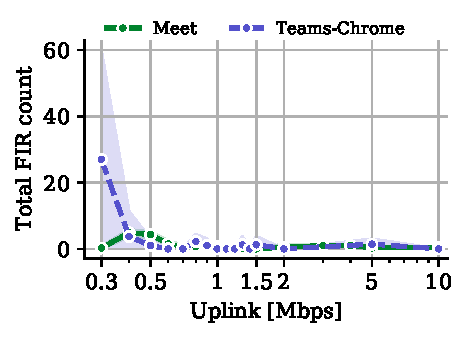
\includegraphics[width=\textwidth]{static/uplink_sent_firCount.pdf}
    \vspace{-1em}
    \caption{Full Intra Request (FIR) count.}
    \label{subfig:uplink_fir}
    \end{subfigure}% 
    \vspace{-1em}
	\caption{Video freeze under downstream and upstream throughput constraints. The bands represent 90\% confidence intervals.%\jamie{These figs are out of scale big}
	}
	\label{fig:video_freeze}
	%\vspace{-1em}
\end{figure}







\subsection{Application Performance}
\label{subsec:application_performance}

Next, we explore how video conference application performance varies depending
on network capacity.  To do so, we rely on the WebRTC stats API
available in Google Chrome to obtain application metrics for \teamsbrowser and
\meet~\cite{webrtc_stats}. We could not obtain the same statistics for
\zoombrowser as it uses DataChannels instead of RTP MediaStream in WebRTC to
transmit media. DataChannels statistics lack any video quality metrics and
mostly contain data volume information. Obtaining application metrics is
challenging for native clients. The Zoom \rev{API}{Web API~\cite{zoom_qos}} does provide limited
application performance (e.g., video resolution, FPS) at a per-minute
granularity for the native client, but this granularity is insufficient to
observe short-term quality fluctuations \rev{}{\footnote{The Zoom native client also provides a statistics tab with fine-grained measures of the same metrics which can be captured using image-based analysis. We consider this as a part of future work}}. We thus limit our analysis in this
section to only \meet and \teamsbrowser. We focus on a subset of metrics
available from WebRTC Stats API that relate to video \textit{quality} and
\textit{freezes}. These metrics are available at a per-second granularity
during each call. 

\paragraph{Video quality}: VCAs adapt the video quality by adjusting the
encoding parameters to achieve a target bitrate estimate provided by the
transport. Ideally, VCAs can adjust one or more of the following three
parameters: 
\begin{itemize}
    \itemsep=-1pt
    \item \emph{frames per second} (FPS), 
    \item \textit{quantization parameter} used in video compression. \rev{}{It regulates the spatial detail saved while encoding the frames. A lower value implies better picture quality}, and  
    \item \textit{video resolution} indicated as the number of pixels in each dimension. In our analysis, we present a single
dimension of the resolution, namely, its \textit{width}. 
\end{itemize}
\noindent

We can obtain all three
parameters from the WebRTC stats. 

We first look at these parameters for different downstream 
capacities
(see~\Cref{subfig:downlink_video_qp,subfig:downlink_frames_per_second,subfig:downlink_frame_width}).
\teamsbrowser simultaneously degrades all three video quality parameters as
downstream capacity decreases. In the case of \teamsbrowser, we also observe
variable behavior across multiple experiments under the same network capacity,
as shown by the $90\%$ confidence interval bands in the plot. \meet, on the
other hand, behaves in a more consistent fashion: it adjusts parameters
differently based on capacity. Within the  0.7--1~Mbps range, \meet adapts the
bitrate primarily by adapting {frames per second}, while keeping the
{quantization parameter} and {frame width} similar to the quality levels in
the absence of degradation. As capacity is further constrained, however,
from 0.5--0.7~Mbps, both the {frame width} and {quantization parameter}
degrade, whereas there is a simultaneous {\em increase} in the frames per
second. Upon closer inspection of the per-second statistics in this operating
range, we find that the relay server may switch to a lower quality copy of the
stream it received via {simulcast}. \meet does not appear to reduce the
bitrate any further by reducing the FPS for the low-quality
stream---specifically, we observed a consistent frame rate even at rates of
less than 0.5~Mbps It is not clear why the quantization parameter reduces
from 38 to 33 at 0.3 Mbps in \meet.

We next analyze the effect of uplink capacity constraints on encoding
parameters
(see~\Cref{subfig:uplink_video_qp,subfig:uplink_frames_per_second,subfig:uplink_frame_width}).
\teams adapts to constrained throughput settings mainly by increasing the
quantization parameter and reducing the frame width, while keeping the FPS
almost constant. To our surprise, we found that the frame width, {\em
increases} as uplink capacity is reduced to 0.3~Mbps.
There seems to be no particularly good explanation for this effect, and (as we
discuss in the next paragraph) it also results in video freezes, suggesting a
poor design decision or implementation bug.  \meet follows a similar trend by
mostly increasing the quantization parameter until the upstream bandwidth
decreases to 0.5 Mbps. At 0.4 Mbps, it also reduces frame width and the FPS. 

\paragraph{Video freezes}: We also analyze the effect of constrained settings
on video freezes. When constraining downlink capacity, we directly obtain the freeze duration
from WebRTC stats. A freeze is assumed to occur if the frame
inter-arrival $>$ max (3$\delta$, $\delta$ + $150 ms$), where $\delta$ is the
average frame duration. We normalize the freeze duration with the total call
duration to obtain freeze ratio.  Figure~\ref{subfig:downlink_freeze_ratio}
shows the freeze ratio under different downstream capacities. The freeze ratio
increases as the downlink bandwidth degrades. \meet has higher freeze ratio than \teamsbrowser with $10\%$ freeze ratio at 0.3~Mbps. Interestingly,
\teamsbrowser incurs freezes (a $3.6\%$ freeze ratio) {\em even in the absence
of throughput constraints}, suggesting again implementation problems or poor
design choices.

When the uplink is constrained, we could not obtain freeze statistics
from V1's logs, because the WebRTC stats provide freeze statistics only for
the received video stream.  Instead, we analyze the total count of Full Intra
Requests (FIR) for the upstream video data. An FIR is sent if the receiver
cannot decode the video or falls behind, likely due to frame losses.  A low
FIR count does not rule out freezes on the receiver, but a high count does
indicate that video freezes are occurring.  Figure~\ref{subfig:uplink_fir}
shows that the FIR count is particularly high for \teamsbrowser at uplink
capacity below 0.5~Mbps. A high FIR count in \teamsbrowser may be triggered
due to the sender sending high-resolution video, as shown in
Figure~\ref{subfig:uplink_frame_width}.


% \textbf{Takeaway}: Uplink 
\vspace{3pt}
\begin{mdframed}[roundcorner=5pt, backgroundcolor=black!10]
\paragraph{Takeaways}: \rev{}{With no constraints on network utilization, 
Zoom and Meet both use under 1~Mbps in both the downlink and uplink directions, 
while Teams uses 1.86/1.40~Mbps. In addition,
VCA performance under the same network conditions varies among the three VCAs. The 
FCC currently recommends a 25/3 Mbps minimum connection. The uplink bandwidth would
be nearly saturated by two simultaneous 2-person Teams call, assuming no background traffic.}
\end{mdframed}

